Reading from a \texttt{csv} file is not always a trivial operation.

Several files contain some heading lines with additional information.
When reading these files it is necessary to apply additional operations to extract these information.

For example, a certain provider exposes market information in different files.
Depending on the file, different operations must be applied.

\paragraph{First rows metadata}
    \begin{figure}
        \centering
        \fbox{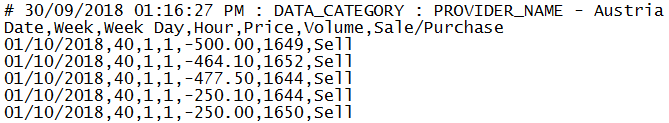
\includegraphics[width=.75\textwidth]{res/etl/epex_ac.PNG}}
        \caption{Metadata in first rows of a \texttt{csv} file.}
        \label{fig:etl:csv:ac}
    \end{figure}
    
    As we can see from Figure \ref{fig:etl:csv:ac}, the first row of the \texttt{csv} file requires special attention.
    
    From it we can extract information about\footnote{
        Some information are under a non-disclosure clause and as such have been anonymized.
    }:
        \begin{itemize}
            \item Creation date \textit{(30/09/2018 01:16:27 PM)}
            \item Category \textit{(DATA\_CATEGORY)}
            \item Provider \textit{(PROVIDER\_NAME)}
            \item Country \textit{(Austria)}
        \end{itemize}
    These information are then appended to each row of the dataset and stored on the Data Warehouse.

\paragraph{Multiple data formats}
    \begin{figure}
        \centering
        \fbox{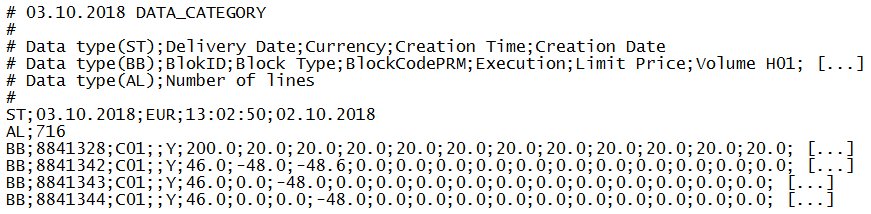
\includegraphics[width=\textwidth]{res/etl/epex_bb.png}}
        \caption{\texttt{Csv} with multiple data formats.}
        \label{fig:etl:csv:bb}
    \end{figure}
    
    For a different data stream, the first 6 rows of the file define some metadata of the dataset, and need to be treated separately.
    Figure \ref{fig:etl:csv:bb} shows the format of the data.
    
    This file contains three different types of data, each with its own format and structure.
    The first rows define the columns available for different types of data.
    The first column of the dataset specifies the data type.
    
    As we can see from Figure \ref{fig:etl:csv:bb}, the first three rows (of type, respectively, \texttt{ST}, \texttt{AL} and \texttt{BB}) have a different number of columns.
    This causes problems when reading the dataset, and requires splitting the file in three datasets, each for a data type.
    
    The first line is, instead, handled similarly to the situation described in the previous example.